
% This LaTeX was auto-generated from an M-file by MATLAB.
% To make changes, update the M-file and republish this document.

\documentclass{article}
\usepackage{graphicx}
\usepackage{color}

\sloppy
\definecolor{lightgray}{gray}{0.5}
\setlength{\parindent}{0pt}

\begin{document}

    
    
\subsection*{Contents}

\begin{itemize}
\setlength{\itemsep}{-1ex}
   \item 1 - Find X, P using Givens and compare.
   \item 2 - Do The Amazing Thing
\end{itemize}
\begin{verbatim}
%%%%%%%%%%%%%%%%%%%%%%%%%%%%%%%%%%%%%%%%%%%%%%%%%%%%%%%%%%%%%%%%%%%%%%%%
%
%
% Zach Dischner-10/31/2012
%
% ASEN 5070-Statistical Orbit Determination
%
% Homework 10
%
% Inputs    : None
%
% Outputs   : Plots for homework 10
%
%
%%%%%%%%%%%%%%%%%%%%%%%%%%%%%%%%%%%%%%%%%%%%%%%%%%%%%%%%%%%%%%%%%%%%%%%%

clc;clear all;close all; format compact;format long g;tic
\end{verbatim}


\subsection*{1 - Find X, P using Givens and compare.}

\begin{verbatim}
e = logspace(-16,-2,1000);

P_Givens    = zeros(2,2,length(e));
P_True      = P_Givens;
X_Givens    = zeros(2,length(e));
tr_Givens   = zeros(length(e),1);
tr_True     = zeros(length(e),1);


Sum_e_squared = zeros(length(e),1);
Sum_e_squared_New = Sum_e_squared;

% Go get plot numbers for the state
for ii = 1:length(e)
    [P_Givens(:,:,ii),X_Givens(:,ii), P_True(:,:,ii),Sum_e_squared(ii),Sum_e_squared_New(ii)] = FindGivens(e(ii));
    tr_Givens(ii)   = trace(P_Givens(:,:,ii));
    tr_True(ii)     = trace(P_True(:,:,ii));
end

% Plot difference in P traces
figure
semilogx(e,abs(tr_Givens - tr_True));
xlabel('\epsilon');ylabel('abs( P Givens - P Batch)'); title('Givens - Batch')
\end{verbatim}

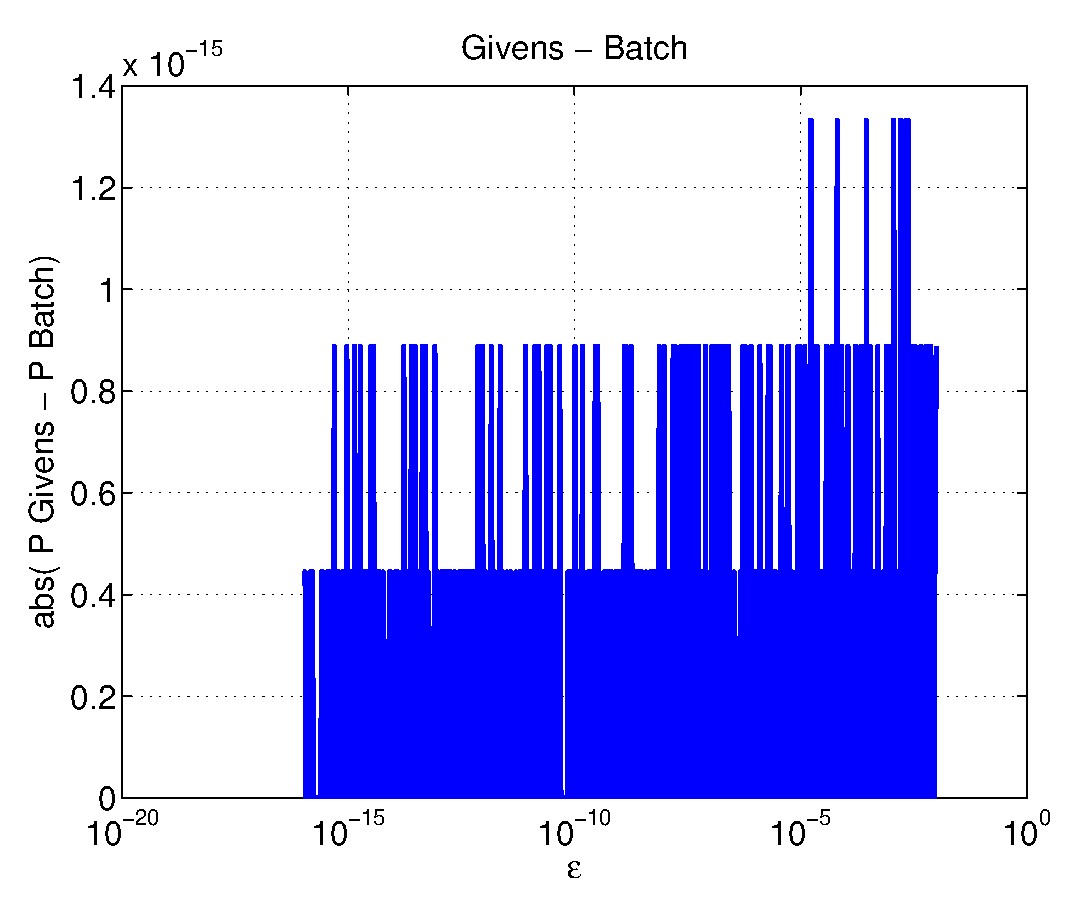
\includegraphics [width=4in]{HW10_01.eps}


\subsection*{2 - Do The Amazing Thing}

\begin{par}
5.4.33 says    sum e\^{}2 = Eta\_hat' * Rbar' * Rbar * Eta\_hat +  sum(/epsilon\^{}2) Eta\_hat = xhat - xbar /epsilon = yi-Hi*xhat
\end{par} \vspace{1em}
\begin{verbatim}
delta = 1e-2;

Rbar    = eye(2,2);
Xbar    = [4;7];
H       = [1 delta;1 1];
y1      = 3;
y2      = 2;

% Xhat = X_Givens(:,1);
[p,Xhat,p2,Sum_e_squared,Sum_e_squared_New]=FindGivens(1e-2);

Eta_hat = Xhat - Xbar;

fprintf('Accumulated e^2 is  :     %3.15f\n\n',Sum_e_squared)

fprintf('EQ 5.4.33  sum e^2  :     %3.15f\n\n',Sum_e_squared_New)

% Make figures awesome and save
figure_awesome('save')
\end{verbatim}

        \color{lightgray} \begin{verbatim}Accumulated e^2 is  :     0.006513006241065

EQ 5.4.33  sum e^2  :     0.006513006241065

\end{verbatim} \color{black}
    
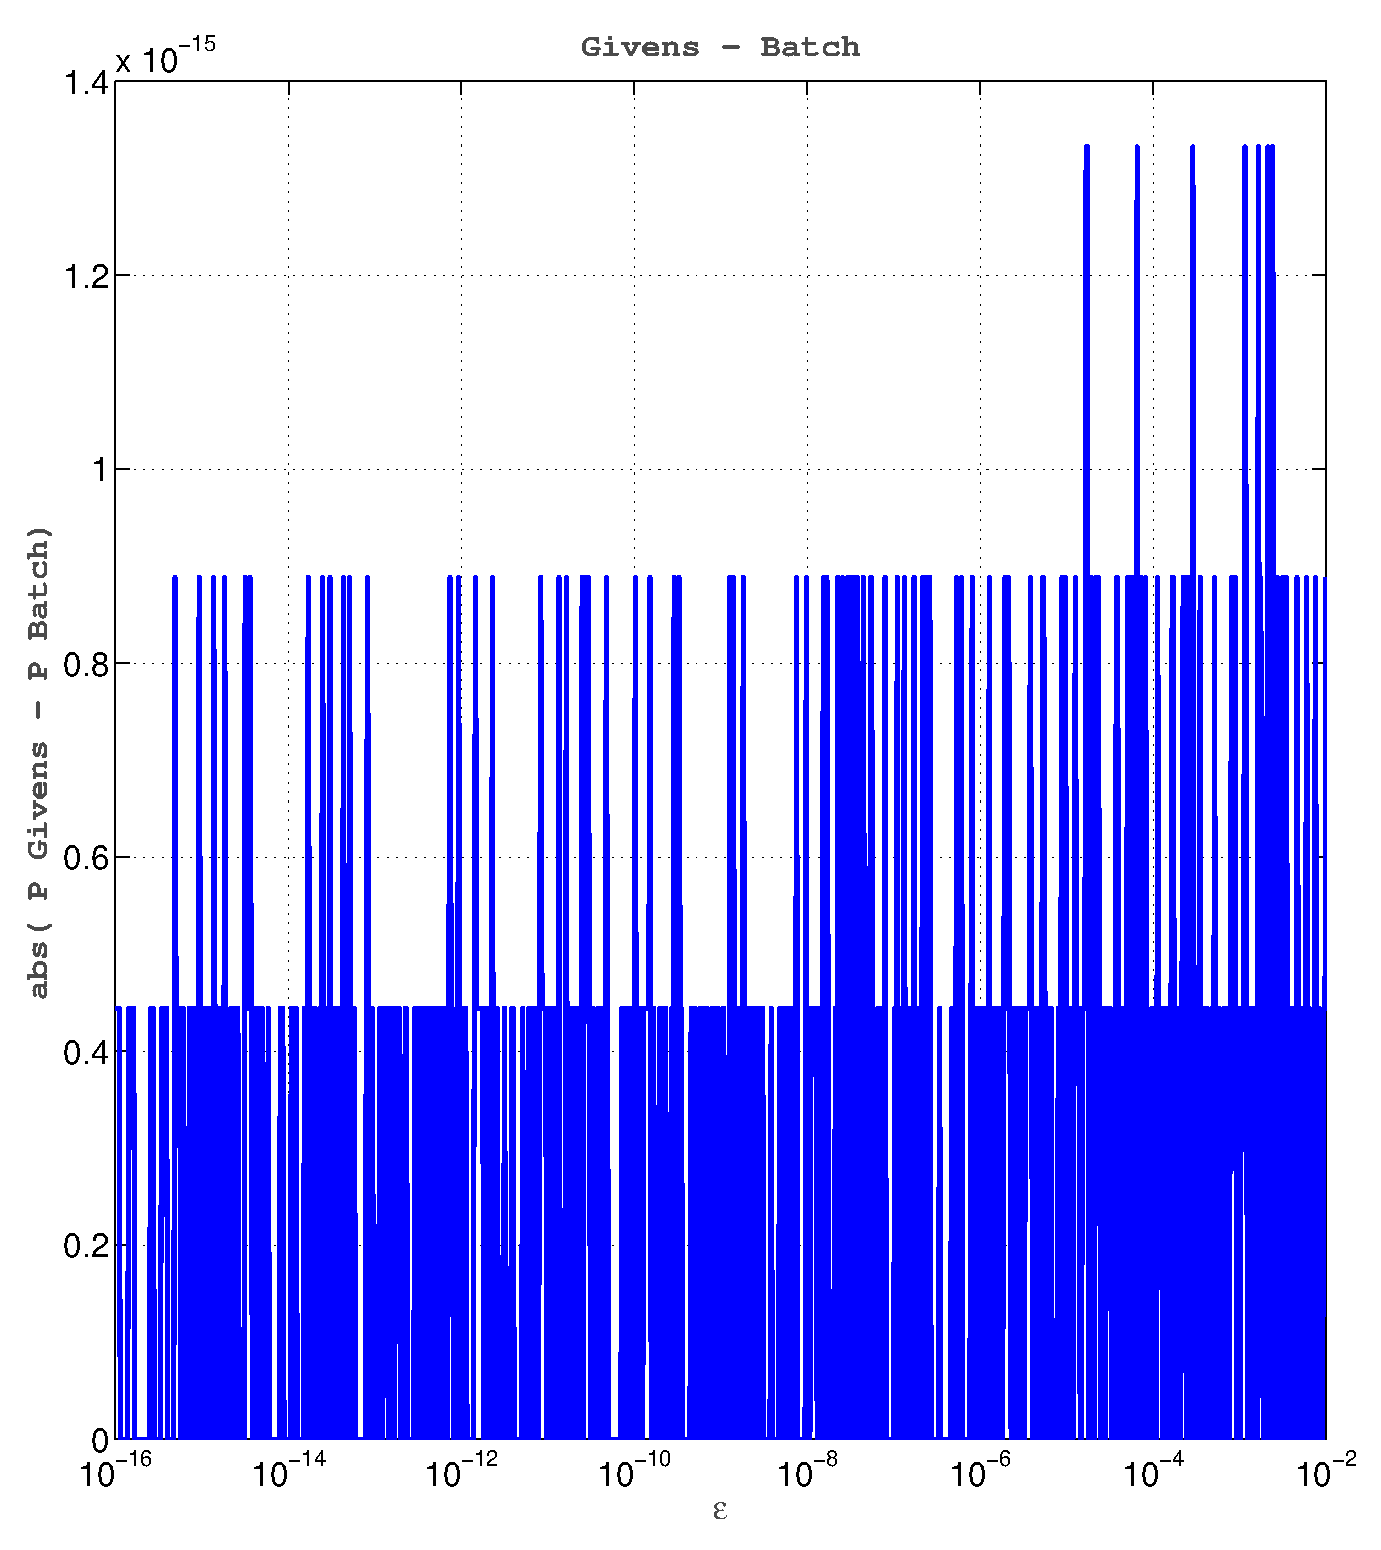
\includegraphics [width=4in]{HW10_02.eps}



\end{document}
    
